\let\negmedspace\undefined
\let\negthickspace\undefined
\documentclass[journal]{IEEEtran}
\usepackage[a5paper, margin=10mm, onecolumn]{geometry}
%\usepackage{lmodern} % Ensure lmodern is loaded for pdflatex
\usepackage{tfrupee} % Include tfrupee package

\setlength{\headheight}{1cm} % Set the height of the header box
\setlength{\headsep}{0mm}     % Set the distance between the header box and the top of the text

\usepackage{gvv-book}
\usepackage{gvv}
\usepackage{cite}
\usepackage{amsmath,amssymb,amsfonts,amsthm}
\usepackage{algorithmic}
\usepackage{graphicx}
\usepackage{textcomp}
\usepackage{xcolor}
\usepackage{txfonts}
\usepackage{listings}
\usepackage{enumitem}
\usepackage{mathtools}
\usepackage{gensymb}
\usepackage{comment}
\usepackage[breaklinks=true]{hyperref}
\usepackage{tkz-euclide} 
\usepackage{listings}
% \usepackage{gvv}                                        
\def\inputGnumericTable{}                                 
\usepackage[latin1]{inputenc}                                
\usepackage{color}                                            
\usepackage{array}                                            
\usepackage{longtable}                                       
\usepackage{calc}                                             
\usepackage{multirow}                                         
\usepackage{hhline}                                           
\usepackage{ifthen}                                           
\usepackage{lscape}
\begin{document}

\bibliographystyle{IEEEtran}
\vspace{3cm}

\title{NCERT - 12.9.6.6}
\author{EE24BTECH11040 - Mandara Hosur}
% \maketitle
% \newpage
% \bigskip
{\let\newpage\relax\maketitle}

\renewcommand{\thefigure}{\theenumi}
\renewcommand{\thetable}{\theenumi}
\setlength{\intextsep}{10pt} % Space between text and floats


\numberwithin{equation}{enumi}
\numberwithin{figure}{enumi}
\renewcommand{\thetable}{\theenumi}

\textbf{Question:}\\
For the differential equation given below, find the general solution:
\begin{align}
x\frac{dy}{dx} + 2y = x^2\ln{x} \label{question}
\end{align}

\textbf{Solution (using the method of finite differences):} \\
A particular solution can be found using the method of finite differences, as illustrated.

\begin{align}
\frac{dy}{dx} = \frac{y(x+h) - y(x)}{h} \\
\implies y(x+h) = y(x) + h\cdot\frac{dy}{dx} \label{difference equation in terms of y}
\end{align}

As can be seen from the question above,

\begin{align}
\frac{dy}{dx} = \frac{x^2\ln{x} - 2y}{x} \\
\implies \frac{dy}{dx} = x\ln{x} - 2\frac{y}{x} \\
\end{align}

Hence, we can rewrite equation \eqref{difference equation in terms of y} as
\begin{align}
\implies y(x+h) = y(x) + h\cdot\brak{x\ln{x} - 2\frac{y}{x}}
\end{align}

Let $x_0 = 0$ and $y_0 = 1$ (assume this as the initial condition as nothing is mentioned in the question). \\
Let some $x_1 = x_0 + h$. Then
\begin{align}
y_1 = y_0 + h\cdot\brak{x_0\ln{x_0} - 2\frac{y_0}{x_0}} \label{initial difference equation}
\end{align}

Iterating through the above-mentioned process to generate $y_2$, $y_3$, $y_4$ and so on generalises equation \eqref{initial difference equation} to

\begin{align}
y_{n+1} = y_n + h\cdot\brak{x_n\ln{x_n} - 2\frac{y_n}{x_n}}
\end{align}

The smaller the value of $h$, the more accurate the curve is. 

\newpage

\textbf{Solution (using manual methods):}

Divide equation \eqref{question} by $x$ in both LHS and RHS.
\begin{align}
\frac{dy}{dx} + \frac{2}{x}y = x\ln{x} \label{linear DE}
\end{align}

This is a linear differential equation. To solve it, we must first calculate its integrating factor ($I.F.$).
\begin{align}
I.F. = e^{\int \frac{2}{x} \,dx} \\
\implies I.F. = e^{2\ln{x}} \\
\implies I.F. = e^{\ln{x^2}} \\
\implies I.F. = x^2 \label{integrating factor}
\end{align}

Multiply equation \eqref{integrating factor} on LHS and RHS of equation \eqref{linear DE}
\begin{align}
\frac{dy}{dx}x^2 + \frac{2}{x}yx^2 = x^3\ln{x} \\
\implies x^2dy + 2xydx = x^3\ln{x}dx \\
\implies D\brak{x^2y} = x^3\ln{x}dx
\end{align}

Integrating on both sides,
\begin{align}
x^2y = \int x^3\ln{x} \,dx \label{calculate RHS}
\end{align}

We can simplify RHS using integration by parts. Let
\begin{align}
u = \ln{x} \text{ , } v = x^3 \label{u and v}
\end{align}
\begin{align}
\implies \frac{du}{dx} = \frac{1}{x} \text{ , } \int v \,dx = \frac{x^4}{4} \label{u and v modif}
\end{align}

According to the rule of integration by parts, 
\begin{align}
\int uv \,dx = u\int v \, dx - \int \brak{\frac{du}{dx} \int v \, dx} \,dx + c \label{integration by parts}
\end{align}
Here $c$ is the constant of integration. \\

Using \eqref{u and v} and \eqref{u and v modif} in \eqref{integration by parts},
\begin{align}
\int x^3\ln{x} \,dx = \frac{x^4}{4}\ln{x} - \int \brak{\frac{1}{x}\cdot\frac{x^4}{4}} \,dx  \\
\implies \int x^3\ln{x} \,dx = \frac{x^4}{4}\ln{x} - \frac{x^4}{16} + c \label{RHS}
\end{align}

Substituting equation \eqref{RHS} in equation \eqref{calculate RHS}, we get
\begin{align}
x^2y = \frac{x^4}{4}\ln{x} - \frac{x^4}{16} + c \\
\implies y = \frac{x^2}{4}\ln{x} - \frac{x^2}{16} + cx^{-2} \label{general form}
\end{align}

Substituting the initial condition of $x=1$, $y=0$ in equation \eqref{general form} gives
\begin{align}
c = \frac{1}{16} \label{c value}
\end{align}

Substituting equation \eqref{c value} in \eqref{general form} gives
\begin{align}
y = \frac{x^2}{4}\ln{x} - \frac{x^2}{16} + \frac{1}{16}x^{-2} \\
\implies y = \frac{x^2}{4}\ln{x} - \frac{1}{16}\brak{x^2 - \frac{1}{x^2}}
\end{align}

Therefore, the equation of the curve found by manual methods is
\begin{align}
y = \frac{x^2}{4}\ln{x} - \frac{1}{16}\brak{x^2 - \frac{1}{x^2}}
\end{align}

\newpage

The curve generated using both described methods for the given question, taking $h=0.1$ and running iterations $100$ times is given below.

\begin{figure}[h]
	\centering
	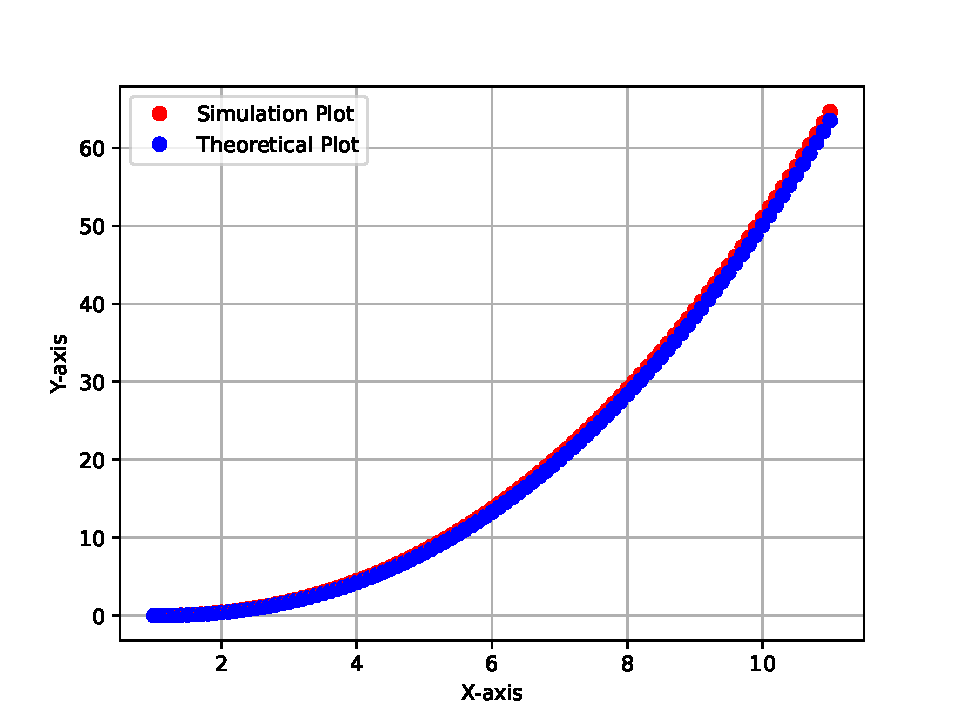
\includegraphics[width=\columnwidth]{figs/fig.pdf}
	\caption{Solution of given DE}
	\label{fig}
\end{figure}

\end{document}
